
%%%%%%%%%%%%%%%%%%%%%%%%%%%%%%%%%%%%%%%%%%%%%%%%%%%%%%%%%%%%%%%%%%%%%%%%%%
%%%%%%%%%%%%%%%%%%%%%%%%%%%%%%%%%%%%%%%%%%%%%%%%%%%%%%%%%%%%%%%%%%%%%%%%%%
\begin{frame}
  \begin{small}
              
  \begin{columns}
  \column{0.9\textwidth}
  \hhref{https://public.wmo.int/en/our-mandate/climate/wmo-statement-state-of-global-climate}{State of Global Climate 2021} report prepared by World Meteorological Organisation (WMO)
    \begin{itemize}\setlength\itemsep{2.0ex}\footnotesize
      \item[o] Annual report detailing the global climate in 2021, including historical comparisons and trends
    \end{itemize}
  \end{columns}

  \end{small}
  \end{frame}

%%%%%%%%%%%%%%%%%%%%%%%%%%%%%%%%%%%%%%%%%%%%%%%%%%%%%%%%%%%%%%%%%%%%%%%%%%%%%%%%%%
\begin{frame}
  \frametitle{\centerline{ \hhref{https://public.wmo.int/en/our-mandate/climate/wmo-statement-state-of-global-climate}{State of Global Climate 2021:} global temperature and CO$_2$ emissions}}
  \begin{scriptsize}

    \begin{columns}
      \column{1.0\textwidth}
      \begin{itemize}\setlength\itemsep{1.3ex}
        \item[o] {\cb Left:} Average global CO$_2$ concentration (parts per million) from 1984 to 2020. The red line is the monthly mean without seasonal variations.

        \item[o] {\it Increasing levels of CO$_2$ and other greenhouse gases in the atmosphere are a major driver of climate change.} Atmospheric CO$_2$ concentrations reflect a balance between emission sources and sinks. Raising global CO$_2$ concentrations reflect the budget between extra emissions due to human activities and uptake by the biosphere and ocean.

        \item[o] {\cb Right:} Mean global temperature from 1850 to 2021. The global temperature in 2021 was $1.11 \pm 0.13~^{\circ}$C above the 1850-1900 average. The six data sets place 2021 between the 5th and 7th warmest year on record. {\it The seven warmest years on record were between 2015 and 2021.}
      \end{itemize}
    \end{columns}

    \begin{columns}

      \column{0.40\textwidth}
        \begin{center}
        {\scriptsize \cb Average global CO$_2$ concentration}
          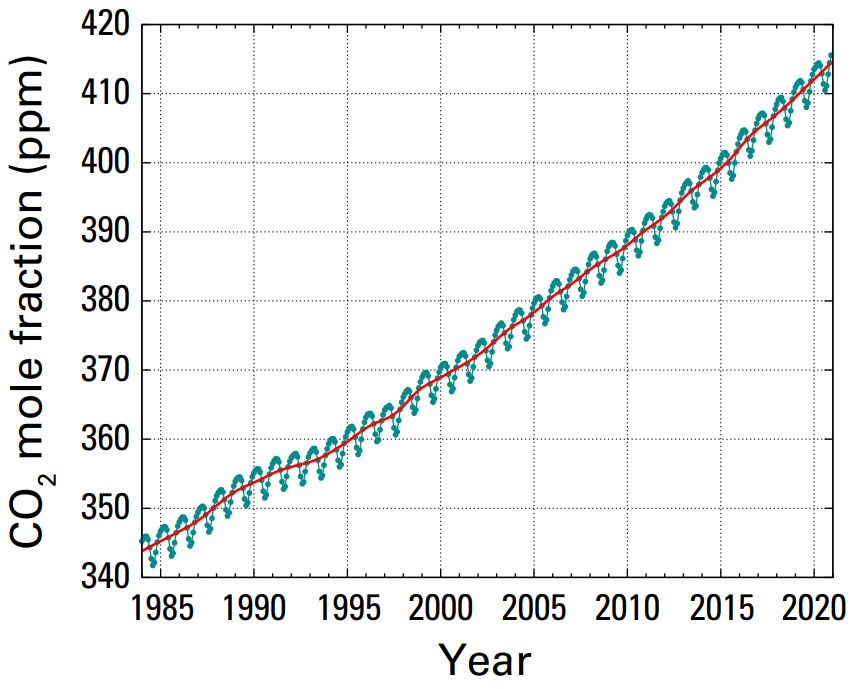
\includegraphics[width=1.0\textwidth]{plots/WMO_CO2}
        \end{center}

      \column{0.65\textwidth}
      \begin{center}
        {\scriptsize \cb Average global temperature change with respect to the 1850-1900 average}
          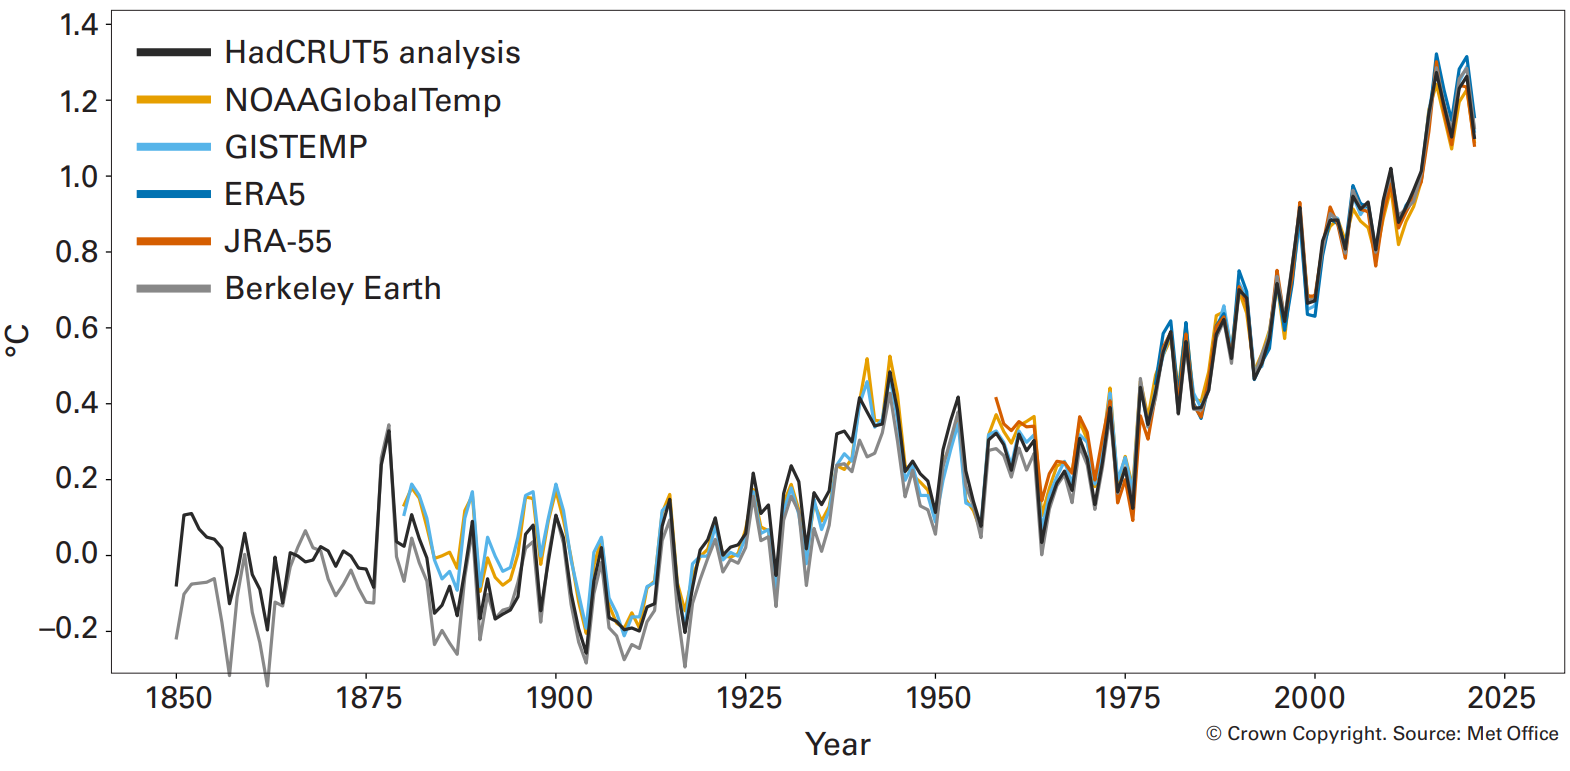
\includegraphics[width=1.0\textwidth]{plots/WMO_temperature}
      \end{center}
    \end{columns}

  \end{scriptsize}
  \end{frame}


%%%%%%%%%%%%%%%%%%%%%%%%%%%%%%%%%%%%%%%%%%%%%%%%%%%%%%%%%%%%%%%%%%%%%%%%%%%%%%%%%%
\begin{frame}
  \frametitle{\centerline{ \hhref{https://public.wmo.int/en/our-mandate/climate/wmo-statement-state-of-global-climate}{State of Global Climate 2021:} average near-surface temperature in 2021}}
  \begin{scriptsize}

    \begin{columns}
      \column{1.0\textwidth}
      \begin{itemize}\setlength\itemsep{1.3ex}
        \item[o] Map of the near-surface temperatures in 2021 compared to the 1981-2010 average. Near-surface temperatures in 2021 were above 1981-2010 average across a broad swath of North America and Greenland, Northern and Tropical Africa, the Middle East and Southern Asia.
        
        \item[o] Cooler conditions in Southern Africa, India, and eastern Australia are characteristic of La Niña. The cooler-than-average area in Northern Asia stands in contrast to 2020, which saw exceptionally high temperatures in the region.

        \item[o] \hhref{https://climate.copernicus.eu/temperature-animations}{Link to animation of year-to-year variations in surface air temperature}
      \end{itemize}
    \end{columns}

    \begin{columns}
      \column{0.7\textwidth}
      \begin{center}
          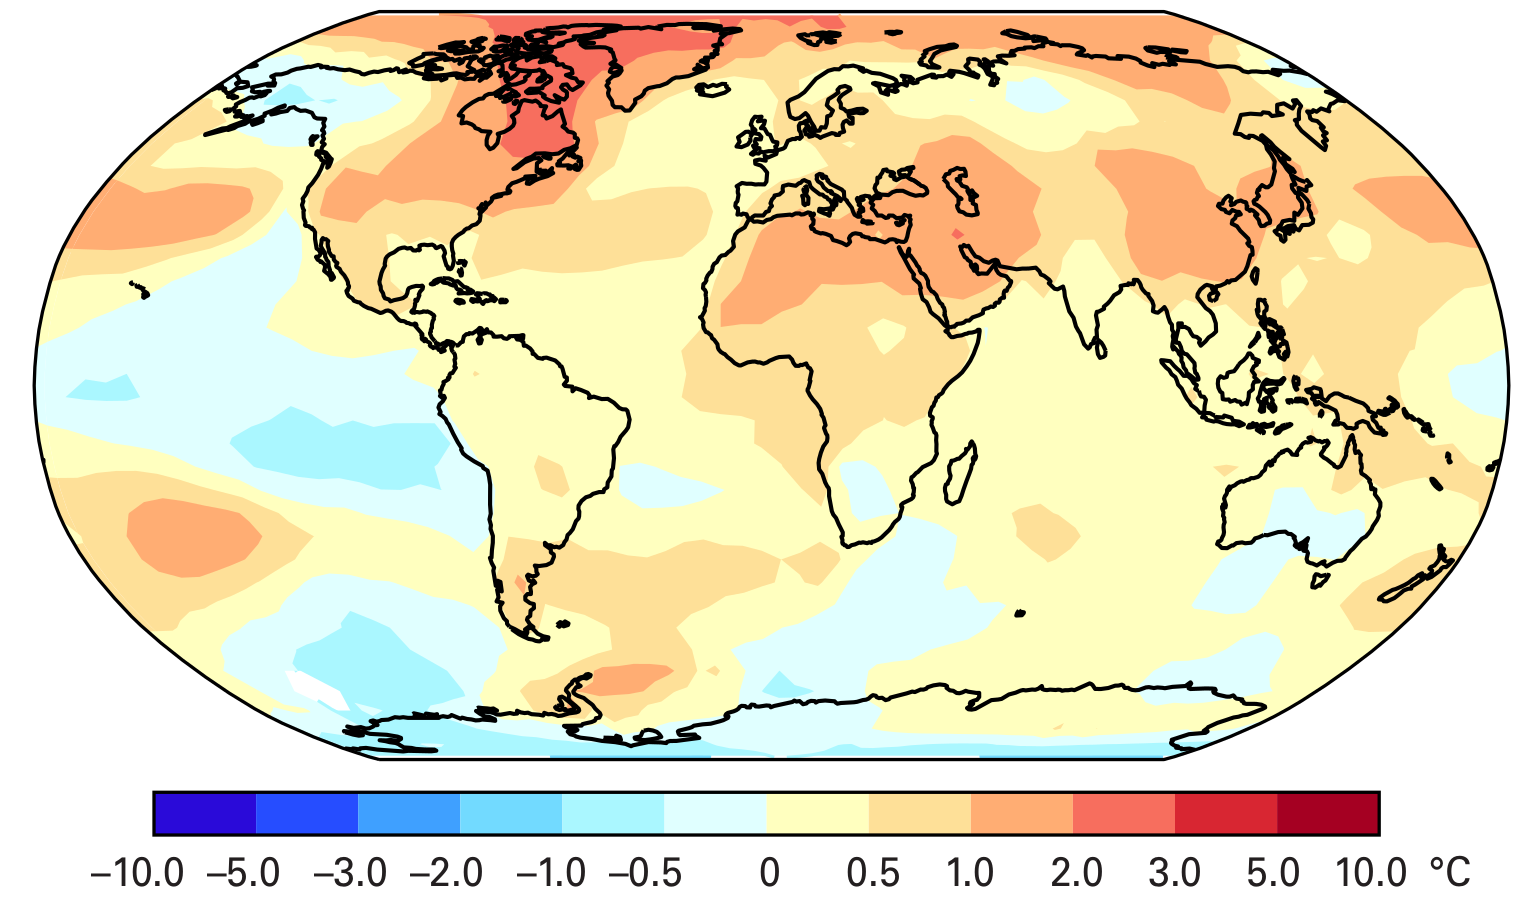
\includegraphics[width=1.0\textwidth]{plots/WMO_temperature_map}
      \end{center}
    \end{columns}

  \end{scriptsize}
  \end{frame}

%%%%%%%%%%%%%%%%%%%%%%%%%%%%%%%%%%%%%%%%%%%%%%%%%%%%%%%%%%%%%%%%%%%%%%%%%%%%%%%%%%
\begin{frame}
  \frametitle{\centerline{ \hhref{https://public.wmo.int/en/our-mandate/climate/wmo-statement-state-of-global-climate}{State of Global Climate 2021:} melting of ice sheets}}
  \begin{scriptsize}

    \begin{columns}
      \column{1.0\textwidth}
      \begin{itemize}\setlength\itemsep{1.3ex}
        \item[o] The average annual rate of ice mass loss from 2002 to 2018 was 276 gigatonne in Greenland and 152 gigatonne in Antarctica, measured with GRACE and GRACE-FO satellite gravity data.        
        \item[o] {\it This is equivalent to about 1.2 mm per year of the global sea-level rise.}

        \item[o] Over the past 30 years, the number of people living in  high risk coastal areas due to rising sea levels increased from 160 million to 260 million.
      \end{itemize}

    \end{columns}

    \vspace{0.2cm}
    \begin{columns}
      \column{1.05\textwidth}
      \begin{center}
          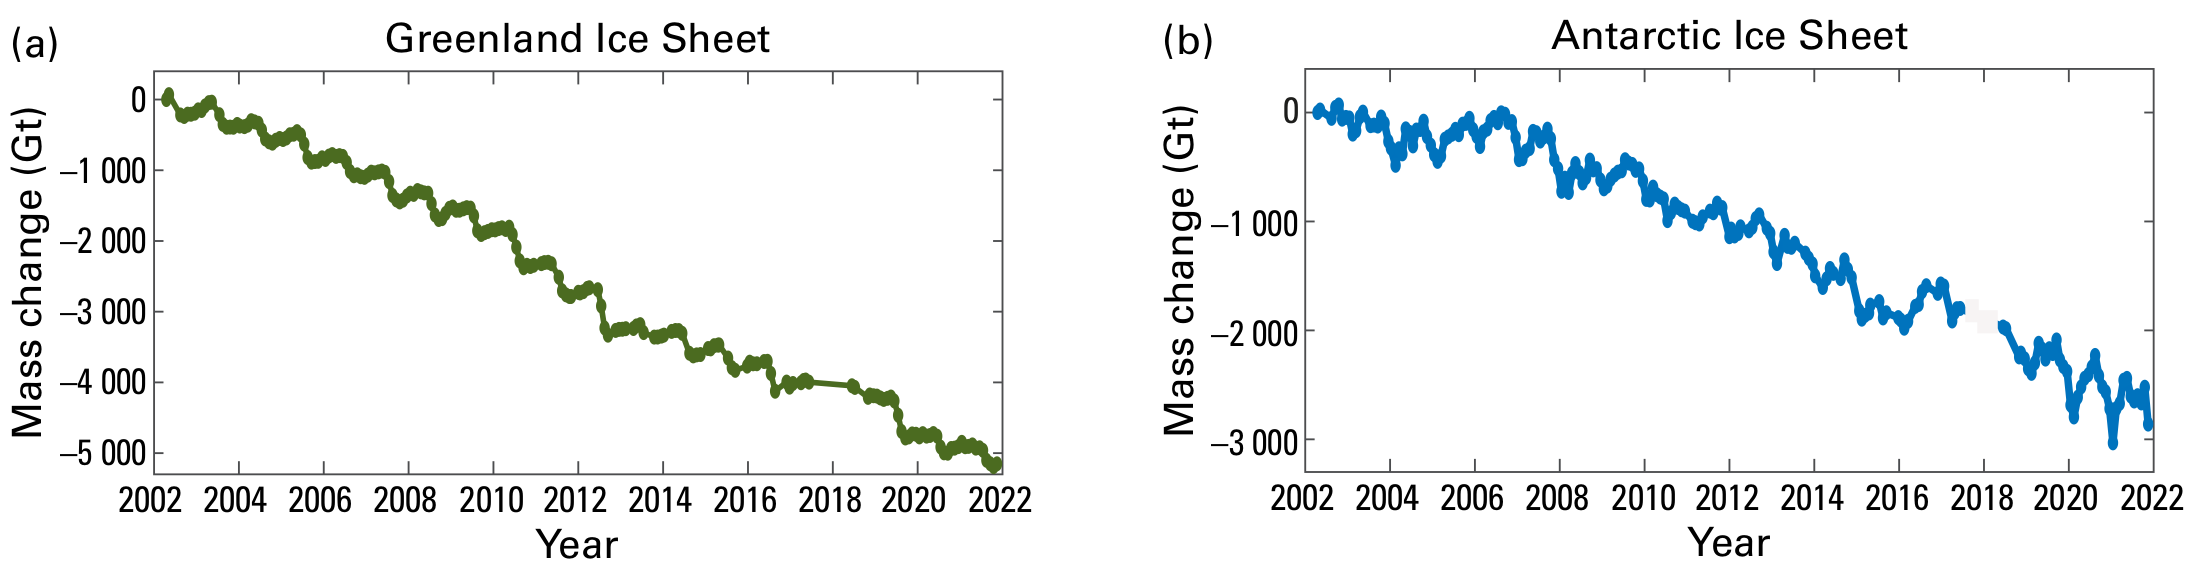
\includegraphics[width=1.0\textwidth]{plots/WMO_ice_sheets}
      \end{center}
    \end{columns}

  \end{scriptsize}
  \end{frame}


%%%%%%%%%%%%%%%%%%%%%%%%%%%%%%%%%%%%%%%%%%%%%%%%%%%%%%%%%%%%%%%%%%%%%%%%%%%%%%%%%%
\begin{frame}
  \frametitle{\centerline{ \hhref{https://public.wmo.int/en/our-mandate/climate/wmo-statement-state-of-global-climate}{State of Global Climate 2021:} see level raise and ocean heat content}}
  \begin{scriptsize}

    \begin{columns}
      \column{1.0\textwidth}
      \begin{itemize}\setlength\itemsep{1.3ex}
        \item[o] {\cb Left:} Global mean sea level evolution from January 1993 to January 2022 (black curve) based on high-precision satellite altimetry. The coloured straight lines represent the average linear trend over three successive time spans: 1993-2002; 2003-2012; 2013-2022.

        
        \item[o] {\cb Right:} Global mean ocean heat content relative to 1955 for depths of 0 to 700~meters in light blue and 700 to 2000~meters in dark blue. 

        \item[o] Oceans cover about 70\% of the earth's surface and have high capacity to absorb extra heat trapped by the CO$_2$ and other greenhouse gases. {\it The ocean takes up more than 90\% of the excess energy accumulating in the Earth climate system as a result of increased concentrations of greenhouse gases.} Melting of ice sheets and thermal expansion of warming oceans lead to a sea level rise, impacting coastlines. Rising CO$_2$ concentrations in the atmosphere change ocean chemistry, causing acidification of the oceans, with negative consequences for marine biosphere.

      \end{itemize}
    \end{columns}

    \begin{columns}
      \column{0.49\textwidth}
      \begin{center}
        {\scriptsize \cb Accelerating raise of the global sea level}
          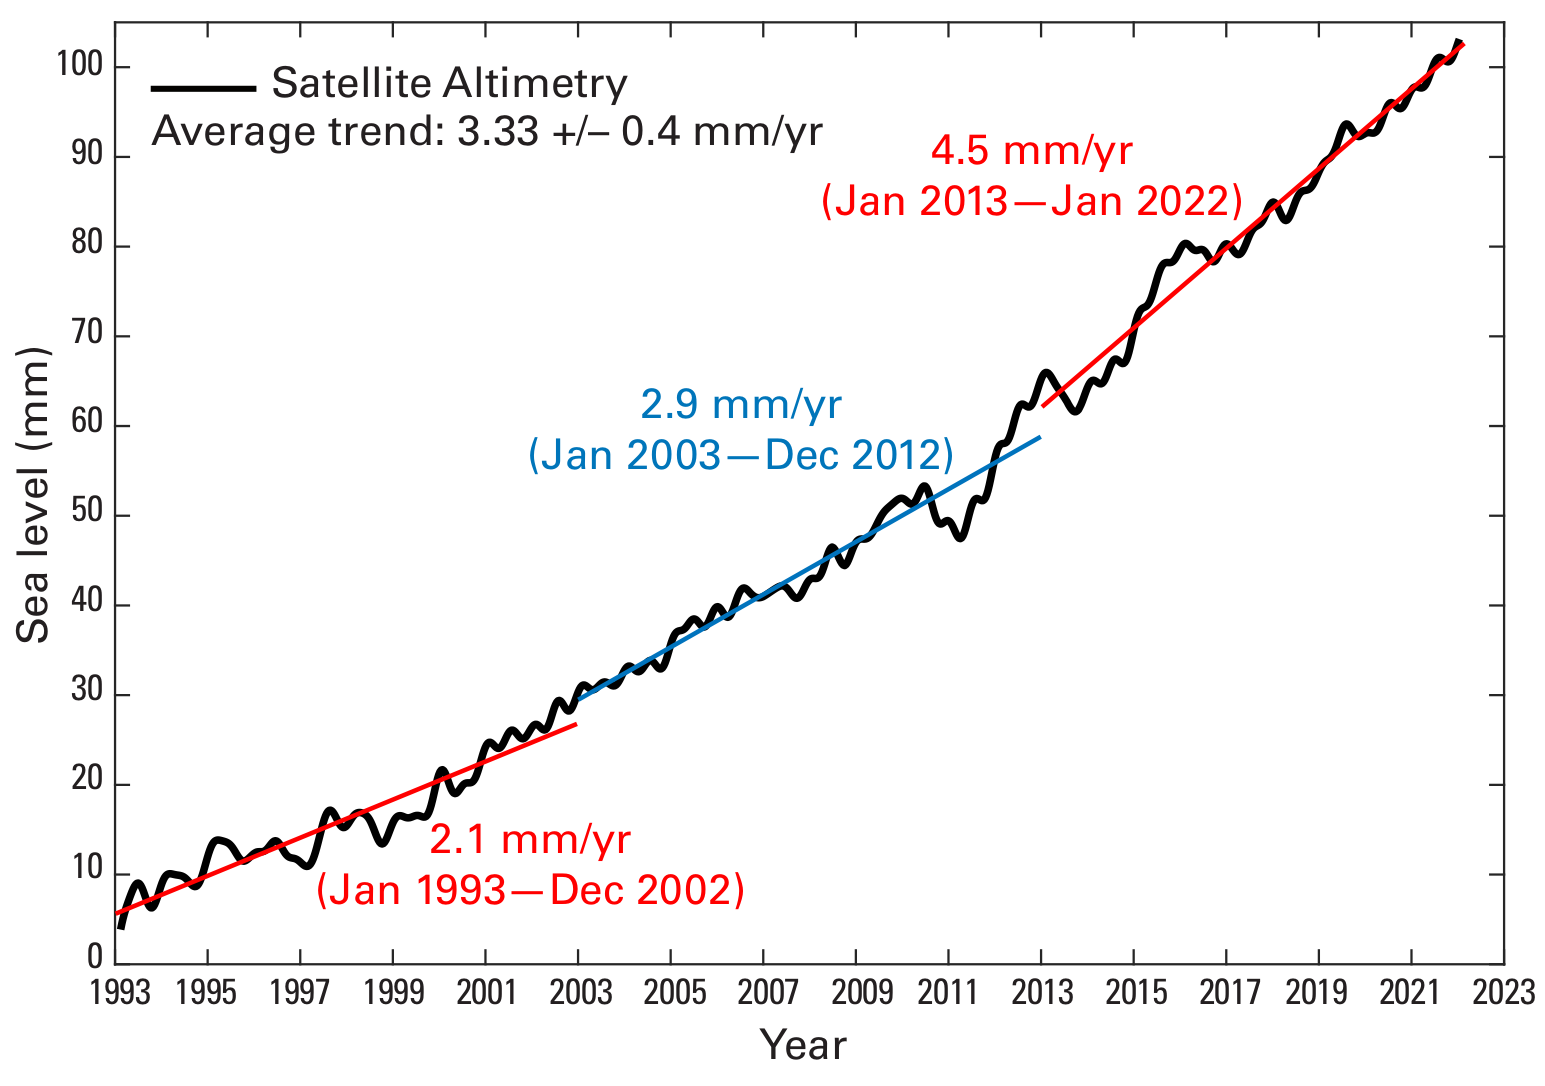
\includegraphics[width=1.0\textwidth]{plots/WMO_sea_level}
      \end{center}

      \column{0.49\textwidth}
      \begin{center}
        {\scriptsize \cb Increasing heat content of the oceans}
          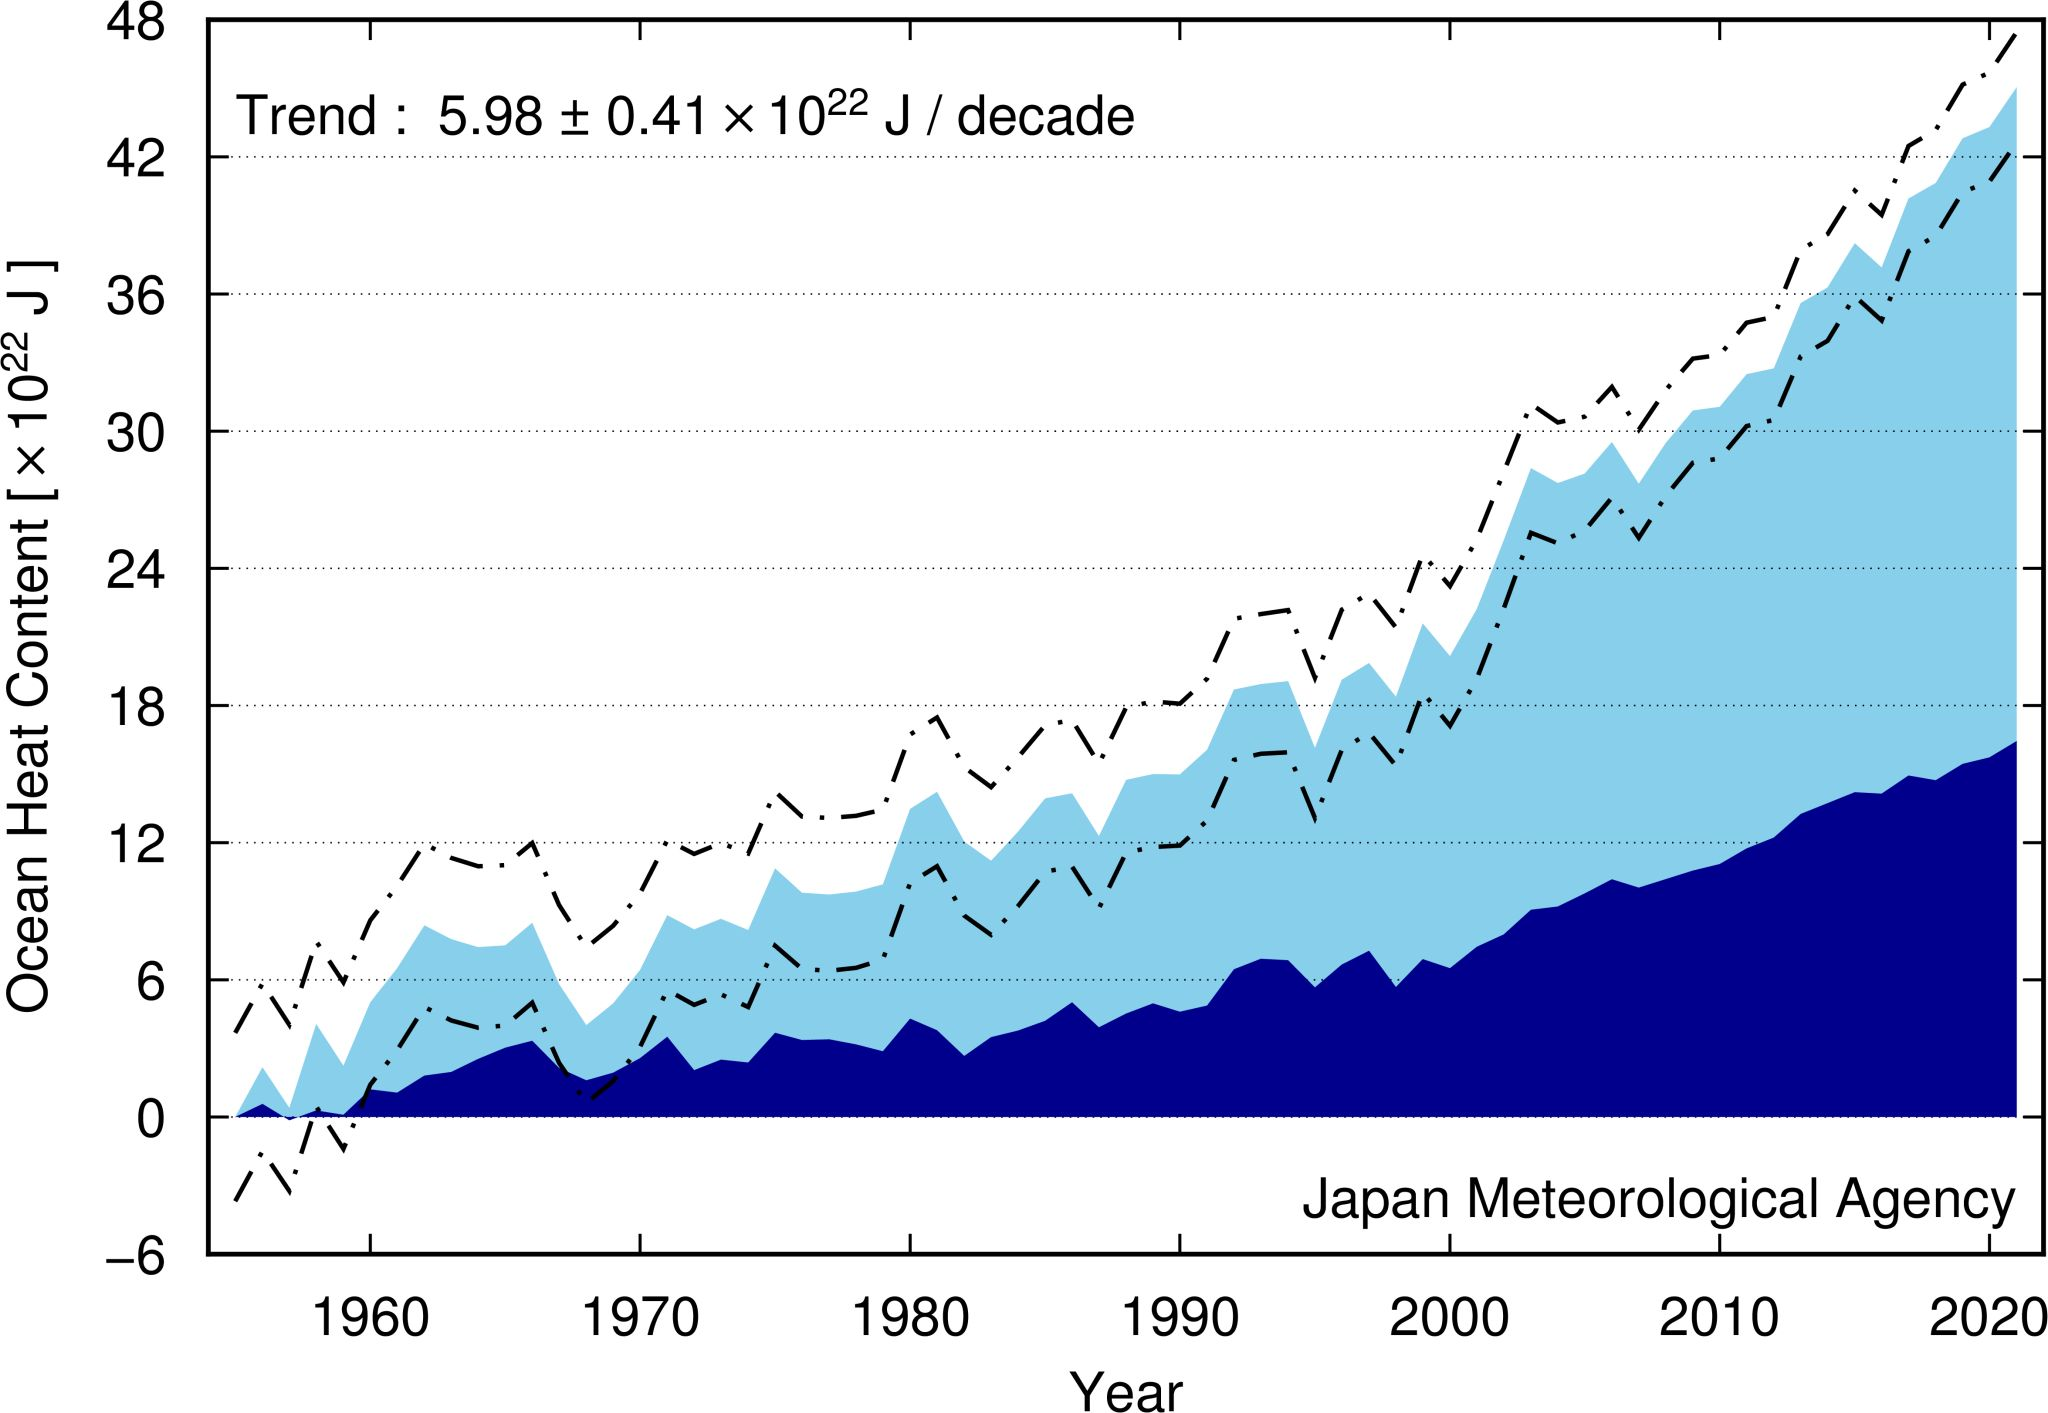
\includegraphics[width=1.0\textwidth]{plots/JMO_sea_heat}
      \end{center}      
    \end{columns}

  \end{scriptsize}
  \end{frame}
